\documentclass[10pt,pscyr]{hedlab}
\usepackage[utf8]{inputenc}
\usepackage[russian]{babel}
\usepackage[derivative,root,shortcuts]{hedmaths}
\usepackage{graphicx}

\usepackage{ucs}
\usepackage{listings}
\lstset{
  extendedchars=\true,
  inputencoding=utf8,
  basicstyle=\footnotesize,
  keepspaces=true,
  breaklines=true,
}
\usepackage[usenames,dvipsnames]{color}
\usepackage[colorlinks,linkcolor=black,citecolor=black,urlcolor=Blue]{hyperref}
\renewcommand{\lstlistingname}{Листинг}

\newcommand{\eq}  [1]{\eqref{eq:#1}}
\newcommand{\pic} [1]{\ref{pic:#1}}
\newcommand{\tab} [1]{\ref{tab:#1}}
\newcommand{\sect}[1]{\ref{sec:#1}}

\student{Чечеткин И. А.}
\date{10.04.2014}
\labname{Сечение упругого рассеяния в борновском приближении}
\labnum{3}

\begin{document}
  \makeheader

  \section{Введение}
  \label{sec:1}
  Множество проблем, связанных со структурой атома может быть количественно
  решено с использованием функции экранирования атома \( \phi(r) \). Эта
  функция определена как отношение между электростатическим потенциалом атома
  \( U(r) \) и электростатическим потенциалом ядра. В атомной системе единиц
  \( \hbar = m = e = 1 \)
  \begin{equation}
    U(r) = -\frac{Z}{r} + \int\limits_0^r \frac{\rho(r')}{r'}\,d^3r'
    \equiv -\frac{Z}{r}\phi(r),
  \label{eq:1}
  \end{equation}
  где \( Z \)~-- заряд ядра, \( \rho(r) \)~-- плотность электронов. Из
  уравнения Пуассона следует, что функция экранирования связана с объемной
  плотностью электронов соотношением 
  \begin{equation}
  \rho(r) = \frac{Z}{4\pi r}\ppder{}{r}\phi(r).
  \label{eq:2}
  \end{equation}
  Большинство из предложенных приблизительных аналитических функций
  экранирования основаны на статистической модели атома Томаса--Ферми (TФ);
  есть только несколько исключений, основанных на самосогласованных
  вычислениях Хартри--Фока (ХФ) или Хартри--Фока--Слейтера (ХФС).
  
  Функции экранирования применяются в модели независимых частиц (МНЧ) при
  вычислении атомной структуры. Одноэлектронные орбитали в МНЧ и энергии связи
  получены решением уравнения Шредингера для потенциала в центральном поле
  \( V(r) \), дающем среднюю энергию взаимодействия атомного электрона,
  находящимся на расстоянии \( r \) от ядра, с зарядом ядра и с другими
  \( Z - 1 \) электронами. Потенциал
  \[
  V(r) = U(r) - V_{ex}(r)
  \]
  отличается от~\eq{1} членом \( V_{ex}(r) \), который учитывает
  обменные эффекты и исключает из \( U(r) \) электростатическое
  взаимодействие каждого электрона с любыми другими электронами~-- обменным
  потенциалом. Обменная поправка обычно представляется с использованием
  аппроксимации Слейтера, то есть из теории свободного электронного газа,
  которая позволяет выразить \( V_{ex}(r) \) через плотность электронов
  \( \rho(r) \):
  \begin{equation}
  V_{ex}(r) = \frac{3}{2}a_X \left(\frac{3}{\pi}\rho(r)\right)^{1/3}.
  \label{eq:4}
  \end{equation}
  Значение параметра \( a_X \) зависит от процедуры, используемой для получения
  \( V_{ex}(r) \) в теории ХФ. Потенциал Слейтера~\eq{4} не адекватен на
  больших расстояниях от ядра. Чтобы гарантировать правильное асимптотическое
  поведение \( V(r) \),
  \[
  rV(r) \to -1 \text{ при } r \to \infty,
  \]
  принимают следующее предложение:
  \begin{equation}
  V(r) = \left\{
  \begin{array}{cl}
  \ds -\frac{Z}{r}\phi(r) - V_{ex}(r), & V(r) < -\frac{1}{r}; \\
  \ds -\frac{1}{r}, & V(r) \ge -\frac{1}{r}
  \end{array}
  \right.
  \label{eq:6}
  \end{equation}
  для вычисления одноэлектронных энергий связи в модели МНЧ для нейтральных
  атомов.
  
  Вычисления Дирака-Хартри-Фока-Слейтера (ДХФС), в которых одноэлектронные
  орбитали являются решением уравнения Дирака вместо уравнения Шредингера,
  включают естественным способом главные релятивистские эффекты на
  одноэлектронных орбиталях и энергиях связи.
  
  В разделе~\sect{2} описана простая аналитическая аппроксимация функции
  экранирования \( \phi_a(r) \) с пятью параметрами, которые определяются по
  результатам вычислений электростатического потенциала атома методом ДХФС.
  Протабулированы параметры для \( Z = 1 \)~-- \( 92 \), полученные из
  самосогласованных результатов ДХФС способом, описанным в разделе~\sect{5}.
  В разделе~\sect{3} атомные форм-факторы и амплитуды рассеяния Борна для
  структурных заряженных частиц, полученных с использованием \( \phi_a(r) \),
  сравниваются с численными результатами, полученными из плотности ДХФС и
  из других аналитических аппроксимаций. Раздел~\sect{4} посвящен анализу
  достоверности результатов МНЧ, основанных на этих функциях экранирования,
  включая сравнения с другими аналитическими потенциалами МНЧ.
  
  \section{Аналитические функции экранирования}
  \label{sec:2}
  Экранирующие функции, применяемые в литературе, обычно основываются на
  модели~ТФ и ее улучшениях. Самая элементарная модель~ТФ дает универсальную
  функцию экранирования, удовлетворяющую следующему дифференциальному
  уравнению:
  \begin{equation}
    \dder{\phi_\text{ТФ}(x)}{x} =
      \frac{\bigl[\phi_\text{ТФ}(x)\big]^{3/2}}{x^{1/2}},
    \label{eq:7}
  \end{equation}
  где \( x = r / b \) с \( b = 0,\!88534 Z^{-1/3} \). Это уравнение не имеет
  аналитического решения, но хорошо аппроксимируется формулой Мольер
  \begin{equation}
    \phi_\text{ТФ}(r) = \sum_{i=1}^3 B_i\exp\bigl(-\beta_i r/b\big),
    \label{eq:8}
  \end{equation}
  где
  \[
    B_1 = 0,\!1, \quad B_2 = 0,\!55, \quad B_3 = 0,\!35, \quad
      \beta_1 = 6,\!0, \quad \beta_2 = 1,\!2, \quad \beta_3 = 0,\!3.
  \]  
  Функция \eq{8} отличается от точного решения уравнения~\eq{7}
  меньше чем на \( 0,\!002 \) в диапазоне \( 0 < x < 6 \).
   
  Потенциал МНЧ может быть представлен также и в следующей аналитической форме:
  \begin{equation}
    V(r) = -\frac{1}{r}\bigl[(Z - 1)\Omega(r) + 1\big],
    \label{eq:9}
  \end{equation}
  где \( \Omega(r) \)~-- функция экранирования с двумя параметрами
  \begin{equation}
    \Omega(r) = \Bigl[H\bigl(e^{r/d} - 1\big) + 1\Big]^{-1},
    \label{eq:10}
  \end{equation}
  где параметры \( H \) и \( d \) вычисляются методом наименьших квадратов для
  потенциала~\eqref{9} применительно к потенциалу ХФС.
  
  Самосогласованные вычисления ДХФС обеспечивают наиболее достоверные функции
  экранирования, учитывающие релятивистские эффекты, которые сложно ввести в
  статистические или самосогласованные нерелятивистские модели. Аппроксимируем
  функцию экранирования ДХФС выражением
  \begin{equation}
    \phi_a(r) = \sum_{i=1}^3 A_i\exp\bigl(-a_i r\big).
    \label{eq:11}
  \end{equation}
  Тогда атомная плотность электронов~\eq{2} принимает вид
  \begin{equation}
    \rho(r) = \frac{Z}{4\pi r} \sum_{i=1}^3 A_i a_i^2\exp\bigl(-a_i r\big).
    \label{eq:12}
  \end{equation}
  Параметры \( A_i \), \( a_i \) были найдены следующим образом. Исходя из
  плотности ДХФС, были вычислены моменты
  \begin{equation}
    R_n \equiv \frac{1}{(n + 1)! Z} \int r^n \rho(r)\,d^3r =
      \frac{1}{(n + 1)!} \int\lni r^{n+1}\dder{\phi(r)}{r}\,dr
    \label{eq:13}
  \end{equation}
  для \( -1 < n < 6 \). Заметим, что с точностью до множителя
  \( 1 / (n + 1)! \), который введен для удобства, величины \( R_n \) совпадают
  с ожидаемыми радиальными значениями \( \average{r^n} \). Легко видеть, что
  \begin{gather*}
    R_{-1} = \der{\phi(0)}{r}, \\
    R_0 = \phi(0), \\
    R_n = \frac{1}{(n - 1)!} \int\lni r^{n-1} \phi(r)\,dr (n \ge 1).
  \end{gather*}
  Параметры функции экранирования~\eq{11}, находились из требования,
  чтобы значения \( R_n \), полученных из нее, совпали с теми, которые
  получены из результатов ДХФС для \( n = -1, 0, 1, 2, 3, 4 \). Это приводит к
  следующим соотношениям:
  \begin{gather}
    A_1 a_1 + A_2 a_2 + A_3 a_3 = R_{-1}, \nonumber \\
    A_1 + A_2 + A_3 = 1, \label{eq:15} \\
    \frac{A_1}{a_1^n} + \frac{A_2}{a_2^n} + \frac{A_3}{a_3^n} = R_n \quad
      (n = 1, 2, 3, 4). \nonumber
  \end{gather}
  При этих условиях гарантируется что:
  \begin{itemize}
    \item \( \ds \der{\phi_a(0)}{r} \) имеет корректное значение
      (совпадающее с ДХФС),
    \item \( \phi_a(0) = 1 \) (только два из трех параметров \( A_i \) должны
      быть даны),
    \item четыре первых момента \( \phi_a(r) \) совпадают с таковыми для
      экранирующей функции ДХФС.
  \end{itemize}
  Последняя особенность делает сечения рассеяния Борна, полученные
  из~\eq{11}, практически совпадающими с вычисленными из экранирующей
  функции ДХФС (см. раздел~\sect{3}).
  
  Для нейтральных атомов уравнение \eq{15} может быть решено аналитически,
  как показано в разделе~\sect{5}. Однако отметим, что значения \( a_i \)
  должны быть положительными, при отрицательных \( a_i \) ожидаемые радиальные
  значения ДХФС не соответствуют условиям \eq{15}, которые, в таком
  случае, должны быть отброшены. Для таких элементов параметры находились из
  четырех первых условий \eq{15}, при этом \( A_3 = 0 \) (см.
  раздел~\sect{5}). Параметры, найденные по этой процедуре для
  \( Z = 1 - 92 \), даны в таблице~\tab{1}. Элементы, обозначенные
  звездочкой, дают ожидаемые радиальные значения ДХФС, противоречащие с
  условиями~\eq{15}.
  
  \begin{table}[!tb]
    \caption{Параметры аналитической функции экранирования \( \phi_a(r) \)}
    \label{tab:1}
    \hspace{-2em}
    \begin{tabular}{|C{.02}|*{5}{>{\(}C{.065}<{\)}|}} \hline
      Z  & A_1       & A_2       & a_1      & a_2      & a_3      \\ \hline
      1  & -184,\!39 & 185,\!39  & 2,\!0027 & 1,\!9973 & 0        \\ \hline
      2  & -0,\!2259 & 1,\!2259  & 5,\!5272 & 2,\!3992 & 0        \\ \hline
      3  & 0,\!6045  & 0,\!3955  & 2,\!8174 & 0,\!6625 & 0        \\ \hline
      4  & 0,\!3278  & 0,\!6722  & 4,\!5430 & 0,\!9852 & 0        \\ \hline
      5  & 0,\!2327  & 0,\!7673  & 5,\!9900 & 1,\!2135 & 0        \\ \hline
      6  & 0,\!1537  & 0,\!8463  & 8,\!0404 & 1,\!4913 & 0        \\ \hline
      7  & 0,\!0996  & 0,\!9004  & 10,\!812 & 1,\!7687 & 0        \\ \hline
      8  & 0,\!0625  & 0,\!9375  & 14,\!823 & 2,\!0403 & 0        \\ \hline
      9  & 0,\!0368  & 0,\!9632  & 21,\!400 & 2,\!3060 & 0        \\ \hline
      10 & 0,\!0188  & 0,\!9812  & 34,\!999 & 2,\!5662 & 0        \\ \hline
      11 & 0,\!7444  & 0,\!2556  & 4,\!1205 & 0,\!8718 & 0        \\ \hline
      12 & 0,\!6423  & 0,\!3577  & 4,\!7266 & 1,\!0025 & 0        \\ \hline
      13 & 0,\!6002  & 0,\!3998  & 5,\!1405 & 1,\!0153 & 0        \\ \hline
      14 & 0,\!5160  & 0,\!4840  & 5,\!8492 & 1,\!1732 & 0        \\ \hline
      15 & 0,\!4387  & 0,\!5613  & 6,\!6707 & 1,\!3410 & 0        \\ \hline
      16 & 0,\!5459  & -0,\!5333 & 6,\!3703 & 2,\!5517 & 1,\!6753 \\ \hline
      17 & 0,\!7249  & -0,\!7548 & 6,\!2118 & 3,\!3883 & 1,\!8596 \\ \hline
      18 & 2,\!1912  & -2,\!2852 & 5,\!5470 & 4,\!5687 & 2,\!0446 \\ \hline
      19 & 0,\!0486  & 0,\!7759  & 30,\!260 & 3,\!1243 & 0,\!7326 \\ \hline
      20 & 0,\!5800  & 0,\!4200  & 6,\!3218 & 1,\!0094 & 0        \\ \hline
      21 & 0,\!5543  & 0,\!4457  & 6,\!6328 & 1,\!1023 & 0        \\ \hline
      22 & 0,\!0112  & 0,\!6832  & 99,\!757 & 4,\!1286 & 1,\!0090 \\ \hline
      23 & 0,\!0318  & 0,\!6753  & 42,\!533 & 3,\!9404 & 1,\!0533 \\ \hline
      24 & 0,\!1075  & 0,\!7162  & 18,\!959 & 3,\!0638 & 1,\!0014 \\ \hline
      25 & 0,\!0498  & 0,\!6866  & 31,\!864 & 3,\!7811 & 1,\!1279 \\ \hline
      26 & 0,\!0512  & 0,\!6995  & 31,\!825 & 3,\!7716 & 1,\!1606 \\ \hline
      27 & 0,\!0500  & 0,\!7142  & 32,\!915 & 3,\!7908 & 1,\!1915 \\ \hline
      28 & 0,\!0474  & 0,\!7294  & 34,\!758 & 3,\!8299 & 1,\!2209 \\ \hline
      29 & 0,\!0771  & 0,\!7951  & 25,\!326 & 3,\!3928 & 1,\!1426 \\ \hline
      30 & 0,\!0400  & 0,\!7590  & 40,\!343 & 3,\!9465 & 1,\!2759 \\ \hline
      31 & 0,\!1083  & 0,\!7489  & 20,\!192 & 3,\!4733 & 1,\!0064 \\ \hline
      32 & 0,\!0610  & 0,\!7157  & 29,\!200 & 4,\!1252 & 1,\!1845 \\ \hline
      33 & 0,\!0212  & 0,\!6709  & 62,\!487 & 4,\!9502 & 1,\!3582 \\ \hline
      34 & 0,\!4836  & 0,\!5164  & 8,\!7824 & 1,\!6967 & 0        \\ \hline
      35 & 0,\!4504  & 0,\!5496  & 9,\!3348 & 1,\!7900 & 0        \\ \hline
      36 & 0,\!4190  & 0,\!5810  & 9,\!9142 & 1,\!8835 & 0        \\ \hline
      37 & 0,\!1734  & 0,\!7253  & 17,\!166 & 3,\!1103 & 0,\!7177 \\ \hline
      38 & 0,\!0336  & 0,\!7816  & 55,\!208 & 4,\!2842 & 0,\!8578 \\ \hline
      39 & 0,\!0689  & 0,\!7202  & 31,\!366 & 4,\!2412 & 0,\!9472 \\ \hline
      40 & 0,\!1176  & 0,\!6581  & 22,\!054 & 4,\!0325 & 1,\!0181 \\ \hline
      41 & 0,\!2257  & 0,\!5821  & 14,\!240 & 2,\!9702 & 1,\!0170 \\ \hline
      42 & 0,\!2693  & 0,\!5763  & 14,\!044 & 2,\!8611 & 1,\!0591 \\ \hline
      43 & 0,\!2201  & 0,\!5618  & 15,\!918 & 3,\!3672 & 1,\!1548 \\ \hline
      44 & 0,\!2751  & 0,\!5943  & 14,\!314 & 2,\!7370 & 1,\!1092 \\ \hline
      45 & 0,\!2711  & 0,\!6119  & 14,\!654 & 2,\!7183 & 1,\!1234 \\ \hline
      46 & 0,\!2784  & 0,\!6067  & 14,\!645 & 2,\!6155 & 1,\!4318 \\ \hline
    \end{tabular}
    \hspace{1em}
    \begin{tabular}{|C{.02}|*{5}{>{\(}C{.065}<{\)}|}} \hline
      Z  & A_1       & A_2       & a_1      & a_2      & a_3      \\ \hline
      47 & 0,\!2562  & 0,\!6505  & 15,\!588 & 2,\!7412 & 1,\!1408 \\ \hline
      48 & 0,\!2271  & 0,\!6155  & 16,\!914 & 3,\!0841 & 1,\!2619 \\ \hline
      49 & 0,\!2492  & 0,\!6440  & 16,\!155 & 2,\!8819 & 0,\!9942 \\ \hline
      50 & 0,\!2153  & 0,\!6115  & 17,\!793 & 3,\!2937 & 1,\!1478 \\ \hline
      51 & 0,\!1806  & 0,\!5767  & 19,\!875 & 3,\!8092 & 1,\!2829 \\ \hline
      52 & 0,\!1308  & 0,\!5504  & 24,\!154 & 4,\!6119 & 1,\!4195 \\ \hline
      53 & 0,\!0588  & 0,\!5482  & 39,\!996 & 5,\!9132 & 1,\!5471 \\ \hline
      54 & 0,\!4451  & 0,\!5549  & 11,\!805 & 1,\!7967 & 0        \\ \hline
      55 & 0,\!2708  & 0,\!6524  & 16,\!591 & 2,\!6964 & 0,\!6814 \\ \hline
      56 & 0,\!1728  & 0,\!6845  & 22,\!397 & 3,\!4595 & 0,\!8073 \\ \hline
      57 & 0,\!1947  & 0,\!6384  & 20,\!764 & 3,\!4657 & 0,\!8911 \\ \hline
      58 & 0,\!1913  & 0,\!6467  & 21,\!235 & 3,\!4819 & 0,\!9011 \\ \hline
      59 & 0,\!1868  & 0,\!6558  & 21,\!803 & 3,\!5098 & 0,\!9106 \\ \hline
      60 & 0,\!1665  & 0,\!7057  & 23,\!949 & 3,\!5199 & 0,\!8486 \\ \hline
      61 & 0,\!1624  & 0,\!7133  & 24,\!598 & 3,\!5560 & 0,\!8569 \\ \hline
      62 & 0,\!1580  & 0,\!7210  & 25,\!297 & 3,\!5963 & 0,\!8650 \\ \hline
      63 & 0,\!1538  & 0,\!7284  & 26,\!017 & 3,\!6383 & 0,\!8731 \\ \hline
      64 & 0,\!1587  & 0,\!7024  & 25,\!497 & 3,\!7364 & 0,\!9550 \\ \hline
      65 & 0,\!1453  & 0,\!7426  & 27,\!547 & 3,\!7288 & 0,\!8890 \\ \hline
      66 & 0,\!1413  & 0,\!7494  & 28,\!346 & 3,\!7763 & 0,\!8969 \\ \hline
      67 & 0,\!1374  & 0,\!7558  & 29,\!160 & 3,\!8244 & 0,\!9048 \\ \hline
      68 & 0,\!1336  & 0,\!7619  & 29,\!990 & 3,\!8734 & 0,\!9128 \\ \hline
      69 & 0,\!1299  & 0,\!7680  & 30,\!835 & 3,\!9233 & 0,\!9203 \\ \hline
      70 & 0,\!1267  & 0,\!7734  & 31,\!681 & 3,\!9727 & 0,\!9288 \\ \hline
      71 & 0,\!1288  & 0,\!7528  & 31,\!353 & 4,\!0904 & 1,\!0072 \\ \hline
      72 & 0,\!1303  & 0,\!7324  & 31,\!217 & 4,\!2049 & 1,\!0946 \\ \hline
      73 & 0,\!1384  & 0,\!7096  & 30,\!077 & 4,\!2492 & 1,\!1697 \\ \hline
      74 & 0,\!1500  & 0,\!6871  & 28,\!630 & 4,\!2426 & 1,\!2340 \\ \hline
      75 & 0,\!1608  & 0,\!6659  & 27,\!568 & 4,\!2341 & 1,\!2970 \\ \hline
      76 & 0,\!1722  & 0,\!6468  & 26,\!586 & 4,\!1999 & 1,\!3535 \\ \hline
      77 & 0,\!1834  & 0,\!6306  & 25,\!734 & 4,\!1462 & 1,\!4037 \\ \hline
      78 & 0,\!2230  & 0,\!6176  & 22,\!994 & 3,\!7346 & 1,\!4428 \\ \hline
      79 & 0,\!2289  & 0,\!6114  & 22,\!864 & 3,\!6914 & 1,\!4886 \\ \hline
      80 & 0,\!2098  & 0,\!6004  & 24,\!408 & 3,\!9643 & 1,\!5343 \\ \hline
      81 & 0,\!2708  & 0,\!6428  & 20,\!941 & 3,\!2456 & 1,\!1121 \\ \hline
      82 & 0,\!2380  & 0,\!6308  & 22,\!987 & 3,\!6217 & 1,\!2373 \\ \hline
      83 & 0,\!2288  & 0,\!6220  & 23,\!792 & 3,\!7796 & 1,\!2534 \\ \hline
      84 & 0,\!1941  & 0,\!6105  & 26,\!695 & 4,\!2582 & 1,\!3577 \\ \hline
      85 & 0,\!1500  & 0,\!6031  & 31,\!840 & 4,\!9285 & 1,\!4683 \\ \hline
      86 & 0,\!0955  & 0,\!6060  & 43,\!489 & 5,\!8520 & 1,\!5736 \\ \hline
      87 & 0,\!3192  & 0,\!6233  & 20,\!015 & 2,\!9091 & 0,\!7207 \\ \hline
      88 & 0,\!2404  & 0,\!6567  & 24,\!501 & 3,\!5524 & 0,\!8376 \\ \hline
      89 & 0,\!2266  & 0,\!6422  & 25,\!684 & 3,\!7922 & 0,\!9335 \\ \hline
      90 & 0,\!2176  & 0,\!6240  & 26,\!554 & 4,\!0044 & 1,\!0238 \\ \hline
      91 & 0,\!2413  & 0,\!6304  & 25,\!193 & 3,\!6780 & 0,\!9699 \\ \hline
      92 & 0,\!2448  & 0,\!6298  & 25,\!252 & 3,\!6397 & 0,\!9825 \\ \hline
    \end{tabular}
  \end{table}
  
  \begin{figure}[htb!]
    \caption{Экранирующие функции для Ne, Zn, и Th (\( Z = 10, 50, \) и
      \( 90 \)). Сплошные кривые~-- результаты ДХФС. Штрихпунктирные и
      штрихованные кривые соответствуют аналитическим функциям экранирования
      \eq{8} и \eq{10} соответственно}
    \label{pic:1}
  \end{figure}
  
  Определенные таким образом аналитические функции экранирования хорошо
  согласуются с результатами ДХФС (рис.~\pic{1}). Естественно, аналитическая
  плотность \eq{12} может только частично воспроизводить колебания плотности
  ДХФС, связанной с различными конфигурациями оболочек (рис.~\pic{2}).
  
  \begin{figure}[htb!]
    \caption{Радиальная плотность для Ar (\( Z = 18 \)). Сплошная кривая~--
      плотность ДХФС. Штрихпунктирная кривая~-- плотность ТФ, полученная из
      функции экранирования Мольер~\eq{8}. Пунктирная кривая соответствует
      плотности, полученной из аналитической функции экранирования~\eq{10}.
      Штриховая кривая~-- аналитическая плотность~\eq{12}}
    \label{pic:2}
  \end{figure}
  
  \section{Упругие сечения Борна}
  \label{sec:3}
  
  Сечение рассеяния Борна для быстрой частицы (которая имеет единичный заряд и
  единичную массу для упрощения) в атомном поле \eq{1} может быть записано как
  \begin{equation}
    \der{\sigma}{\Omega} = \frac{4Z^2}{q^4} \left[1 - \frac{F(q)}{Z}\right]^2,
    \label{eq:16}
  \end{equation}
  где \( q \)~-- переданный импульс в столкновении и
  \begin{equation}
    F(q) = \int\lni \frac{\sin(qr)}{qr} \rho(r) 4\pi r^2\,dr
    \label{eq:17}
  \end{equation}
  -- атомный форм-фактор. Для плотности, связанной с аналитическими
  экранирующими функциями, форм-фактор принимает простое выражение
  \begin{equation}
    \frac{F(q)}{Z} = \sum\limits_{i=1}^3 \frac{A_i a_i^2}{a_i^2 + q^2}.
    \label{eq:18}
  \end{equation}
  Раскладывая правую часть уравнения \eq{17} в ряд по степеням \( q \), находим
  \[
    \frac{F(q)}{Z} = \sum\limits_{n=0}^\infty (-1)^n R_{2n} q^{2n},
  \]
  с коэффициентами \( R_n \), данными в~\eq{13}. Очевидно, с параметрами
  аналитической экранирующей функции, удовлетворяющей~\eq{15}, мы гарантируем,
  что атомный форм-фактор~\eq{18} и его первые производные совпадают при
  \( q = 0 \) с теми, которые вычислены из плотности ДХФС.
  
  \begin{figure}[htb!]
    \caption{Атомные форм-факторы для Sn (\( Z = 50 \)). Сплошная кривая~--
      форм-фактор ДХФС. Штрихпунктирная кривая~-- форм-фактор, полученный из
      функции экранирования Мольер~\eq{8}. Пунктирная кривая соответствует
      форм-фактору, полученному из аналитической функции экранирования~\eq{10}.
      Штриховая кривая~-- форм-фактор, полученный из функции
      экранирования~\eq{11}}
    \label{pic:3}
  \end{figure}
  
  Форм-факторы~\eq{18} сравниваются с полученными из плотности ДХФС, и из
  других аналитических функций экранирования на рис.~\pic{3} для \( Z = 50 \).
  Аналитические результаты отличаются от численных вычислений ДХФС только для
  относительно больших переданных импульсов. Хотя эти различия могли бы
  показаться важными, они незначительно влияют на результирующее
  дифференциальное сечение рассеяния Борна (см. рис.~\pic{4} и~\pic{5}),
  которое определятся только квадратом разности
  \( \bigl[1 - F(q) / Z\big]^2 \) с весом \( q^{-4} \).
  
  \begin{figure}[htb!]
    \caption{Дифференциальное сечение рассеяния Борна для Sn (\( Z = 50 \)).
      Штрихпунктирные кривые и штриховые кривые были получены из аналитических
      функций экранирования~\eq{8} и~\eq{10}, соответственно. Сплошная кривая~--
      сечение ДХФС. Сечение рассеяния, полученное из аналитической
      плотности~\eq{12} совпадает с ДХФС на рисунке}
    \label{pic:4}
  \end{figure}
  
  \begin{figure}[htb!]
    \caption{Дифференциальные сечения рассеяния Борна для Zn (\( Z = 30 \)).
      Сплошная кривая~-- сечение ДХФС. Соответствие между кривыми и
      теоретическими моделями, из которых они были получены, такое же, как и
      на рис.~\pic{4}; здесь сечение рассеяния, полученное из аналитической
      плотности~\eq{10} показывается кривой с короткими штрихами}
    \label{pic:5}
  \end{figure}
  
  Полное сечение рассеяния Борна для энергии \( E \) падающей частицы получают
  интегрированием дифференциального сечения~\eq{16} 
  \[
    \int\,d\Omega\der{\sigma}{\Omega} = \int\limits_0^{2\pi} d\phi
      \int\limits_0^\pi \sin\theta\,d\theta \frac{4Z^2}{q^4}
      \left[1 - \frac{F(q)}{Z}\right]^2.
  \]
  
  \begin{figure}[htb!]
    \caption{Схема упругого столкновения}
    \label{pic:6}
  \end{figure}
  
  Как можно видеть из приведенной на рис.~\pic{6} схемы столкновения,
  переданный импульс \( q \) связан с импульсом рассеивающегося на атоме
  электрона \( k = \bigl(2E\big)^{1/2} \) и углом рассеяния \( \theta \)
  соотношением
  \[
    \frac{q}{2} = k\sin\frac{\theta}{2},
  \]
  которое может быть переписано как
  \[
    \left(\frac{1}{2k}\right)^2 = \sin^2\frac{\theta}{2} = \frac{1}{2}
      \bigl(1 - \cos\theta\big).
  \]
  Переходя в интеграле от переменной \( \theta \) к переменной \( q \), получим
  \[
    \sigma(E) = \frac{4\pi}{E}Z^2 \int\limits_0^{(8E)^{1/2}} \frac{1}{q^3}
      \left(1 - \frac{F(q)}{Z}\right)^2\,dq.
  \]

  Различия между полными сечениями рассеяния, полученными из различных
  экранирующих функций, показаны на рис.~\pic{6}, где \( \sigma E \) показана
  как функция импульса частицы \( k = \bigl(2E\big)^{1/2} \). Очевидно,
  что форм-факторы, чьи производные при \( q = 0 \) отличаются незначительно,
  но очень похожи, могут давать весьма различные сечения рассеяния. В
  частности, экранирующая функция ТФ очень неудовлетворительно описывает
  упругие столкновения; это последствие нереалистично большого хвоста
  электронной плотности ТФ.
  
  \begin{figure}[htb!]
    \caption{Полные сечения рассеяния Борна как функции импульса \( k \)
      падающей частицы (умноженного на \( E = k^2 / 2 \)) для Sn (\( Z = 50 \)).
      Соответствие между кривыми и различными экранирующими функциями, из
      которых они были получены, такое же, как на рис.~\pic{4}}
    \label{pic:6}
  \end{figure}
  
  \section{Вычисления МНЧ}
  \label{sec:4}
  
  В контексте нерелятивистской МНЧ свойства атома получены решением уравнение
  Шредингера для занятых одноэлектронных орбиталей. Релятивистская МНЧ
  основывается на тех же принципах, за исключением того факта, что
  одноэлектронные орбитали и энергии связи найдены из решения уравнения Дирака.
  Вследствие сферической симметрии потенциала, могут быть приняты орбитали в
  центральном поле и их радиальные части, полученные из решения соответствующих
  радиальных уравнений. Они могут быть численно решены с использованием
  стандартных численных методов.
  
  Достоверность аналитических экранирующих функций, принятых за основу для
  вычислений МНЧ, демонстрируется в таблице~\tab{2}, где экспериментальные и
  энергии связи ДХФС сравниваются с полученными из релятивистской МНЧ с
  экранирующими функциями (используя~\eq{6} как потенциал МНЧ). Подобное
  согласие найдено между орбиталями МНЧ и ДХФС. Нерелятивистские энергии связи,
  полученные из вычислений ХФС и из МНЧ, используя потенциал~\eq{9}, с
  параметрами, полученными подгонкой экспериментальных энергий ионизации
  (исправленными для релятивистских эффектов), также показаны в таблице~\tab{2}.

  \begin{table}[!tb] % почему таблицы уезжают на отдельные страницы???
    \center
    \caption{Собственные значения энергии и ожидаемые радиальные значения для
      олова (\( Z = 50 \)) (в атомных единицах). Expt.: экспериментальные
      данные. ДХФС: релятивистские самосогласованные результаты. МНЧ:
      релятивистские собственные значения из аналитической экранирующей функции.
      ХФС: нерелятивистские вычисления ХФС. GSZ: получены из аналитического
      потенциала~\eq{9}. Сравнение ожидаемых радиальных значений плотностей
      ДХФС и ХФС ясно показывает, что релятивистские эффекты имеют тенденцию
      концентрировать электронное облако около ядра}
    \label{tab:2}
    \begin{tabular}{*{6}{>{\(}C{.1}<{\)}}} \hline
                       & \text{Expt.} & \text{ДХФС} & \text{МНЧ} & \text{ХФС} &
        \text{GSZ} \\ \hline
      1s_{1/2}         & 1073.08      & 1072.51     & 1067.64    & 1034.54    &
        1042.54    \\
      2s_{1/2}         & 164.07       & 163.18      & 161.27     & 153.92     &
        156.44     \\
      2p_{1/2}         & 152.73       & 152.91      & 149.97     & 144.42     &
        147.70     \\
      2p_{3/2}         & 144.38       & 144.29      & 141.57     &            &
                   \\
      3s_{1/2}         & 34.68        & 31.93       & 32.25      & 30.04      &
        30.74      \\
      3p_{1/2}         & 29.84        & 27.68       & 27.95      & 26.05      &
        26.87      \\
      3p_{3/2}         & 26.25        & 26.09       & 26.34      &            &
                   \\
      3d_{3/2}         & 18.13        & 18.49       & 18.95      & 18.58      &
        19.36      \\
      3d_{5/2}         & 17.82        & 18.16       & 17.24      &            &
                   \\
      4s_{1/2}         & 5.02         & 5.24        & 5.16       & 4.88       &
        5.16       \\
      4p_{1/2}         & 3.26         & 3.80        & 3.71       & 3.53       &
        3.82       \\
      4p_{3/2}         & 3.51         & 3.43        &            &            &
                   \\
      4d_{3/2}         & 0.88         & 1.22        & 1.18       & 1.26       &
        1.51       \\
      4d_{5/2}         & 1.17         & 1.14        &            &            &
                   \\
      5s_{1/2}         & 0.48         & 0.49        & 0.46       & 0.53       &
                   \\
      5p_{1/2}         & 0.23         & 0.22        & 0.22       & 0.57       &
                   \\ \hline
      \average{r^{-1}} &              & 302.20      &            & 288.59     &
                   \\
      \average{r^{-2}} &              & 56.55       &            & 58.87      &
                   \\
      \average{r^{-4}} &              & 629.87      &            & 701.33     &
                   \\ \hline
    \end{tabular}
  \end{table}
  
  Таблица~\tab{2} включает ожидаемые радиальные значения \( \average{r^{-1}} \),
  \( \average{r^{-2}} \) и \( \average{r^{-4}} \), вычисленные из
  самосогласованных плотностей ДХФС и ХФС. Существуют явные различия между
  ожидаемыми значениями ДХФС и ХФС, являющиеся результатом релятивистских
  поправок, ведущих к концентрации электронного заряда около ядра. Как
  следствие, экранирующая функция ДХФС с увеличением радиальных расстояний
  уменьшается быстрее, чем экранирующая функция ХФС. Эти релятивистские эффекты
  на экранирующих функциях не могут быть посчитаны, если релятивистские
  поправки представлены возмущенными нерелятивистскими одноэлектронными
  орбиталями.
  
  \section{Приложение}
  \label{sec:5}
  
  Уравнения~\eq{15} могут быть аналитически решены для параметров экранирующей
  функции. После алгебраических манипуляций можно избавиться от констант
  \( A_i \); результирующие уравнения для \( a_i \) могут быть записаны в форме
  \begin{gather}
    R_{-1} - (a_1 + a_2 + a_3) + R_1(a_1 a_2 + a_1 a_3 + a_2 a_3) -
      R_2 a_1 a_2 a_3 = 0, \nonumber \\
    1 - R_1(a_1 + a_2 + a_3) + R_2(a_1 a_2 + a_1 a_3 + a_2 a_3) -
      R_3 a_1 a_2 a_3 = 0, \label{eq:A1} \\
    R_1 - R_2(a_1 + a_2 + a_3) + R_3(a_1 a_2 + a_1 a_3 + a_2 a_3) -
      R_4 a_1 a_2 a_3 = 0. \nonumber
  \end{gather}
  Эти уравнения теперь могут быть решены для величин
  \begin{gather*}
    \alpha_2 = a_1 + a_2 + a_3, \\
    \alpha_1 = a_1 a_2 + a_1 a_3 + a_2 a_3, \\
    \alpha_0 = a_1 a_2 a_3.
  \end{gather*}
  
  Таким образом, параметры экранирующей функции \( a_i \) (\( i = 1, 2, 3 \))~--
  три решения кубического уравнения
  \begin{equation}
    a^3 + \alpha_2 a^2 + \alpha_1 a + \alpha_0 = 0.
    \label{eq:A3}
  \end{equation}
  Если три корня~\eq{A3} действительны и положительны, параметры \( A_i \)
  могут тогда быть вычислены из первых трех уравнений~\eq{15}. 
  В некоторых случаях, главным образом для малых атомных чисел,
  условия~\eq{15} несовместны с ожидаемыми радиальными значениями ДХФС
  \( R_n \), то есть, или определитель матрицы~\eq{A1} равен нулю, или
  некоторые из корней~\eq{A3} комплексные. В этих случаях продолжать вычисления
  следует так, как показано в разделе~\sect{2}, то есть полагать \( A_3 = 0 \)
  и налагать только первые четыре условия~\eq{15}. Выполняя те же самые
  действия, как и в вышеупомянутом вычислении, легко показать, что \( a_1 \) и
  \( a_2 \) могут быть получены как решения квадратного уравнения
  \[
    \bigl(R_2 - R_1^2\big) a^2 + \bigl(R_1 - R_{-1}R_2\big)a +
      \bigl(R_{-1} R_2 - 1\big) = 0
  \]
  и
  \[
    A_1 = \frac{R_{-1} - a_2}{a_1 - a_2}, \qquad A_2 = 1 - A_1.
  \]
  Отметим что даже когда уравнения~\eq{15} несовместимы, форм-фактор~\eq{18},
  и, по крайней мере, три его первые производные совпадают при \( q = 0 \) с
  вычисленными из самосогласованной плотности ДХФС.

  \section{Численное решение}
  \label{sec:6}
%  \begin{figure}[h!]
%  \vspace{-1em} \hspace{-2em}
%  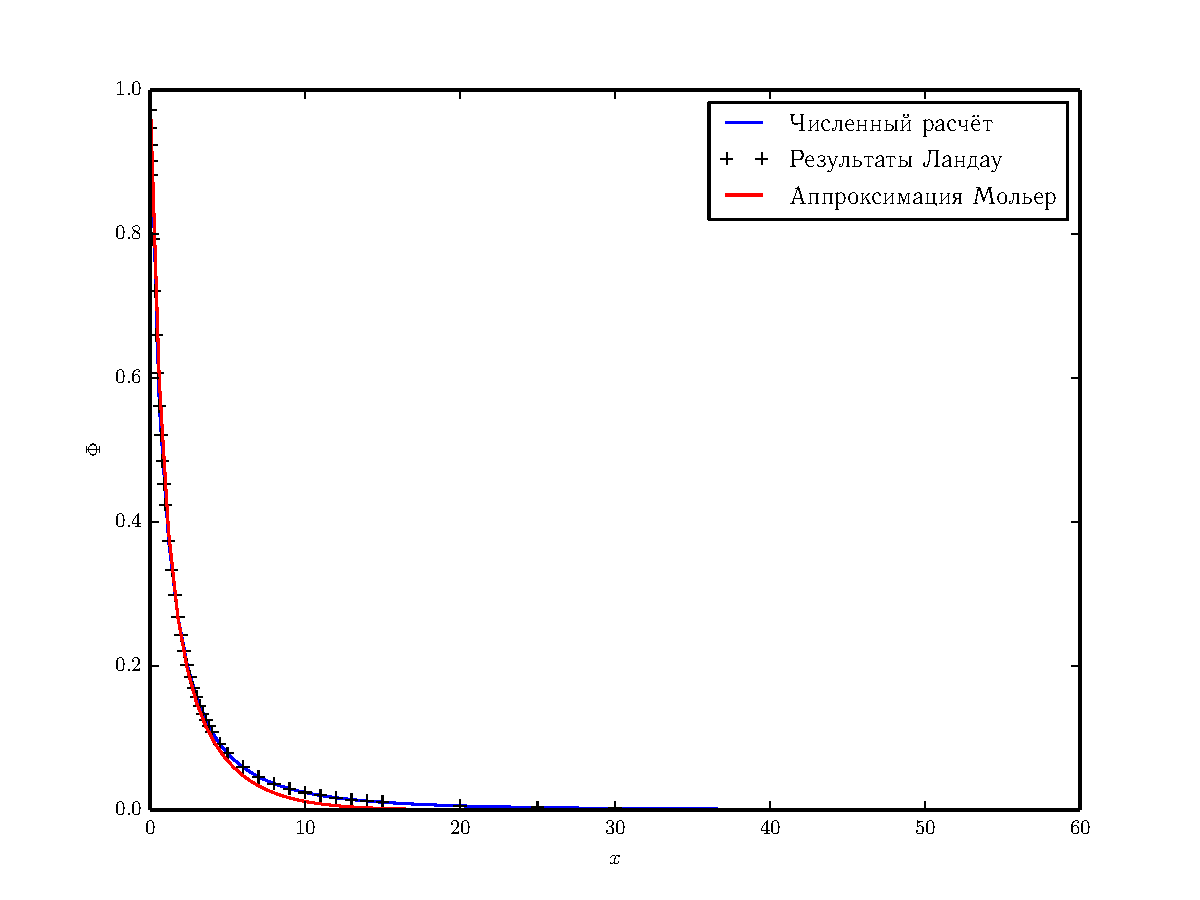
\includegraphics[width=.55\textwidth]{common} \hspace{-3em}
%  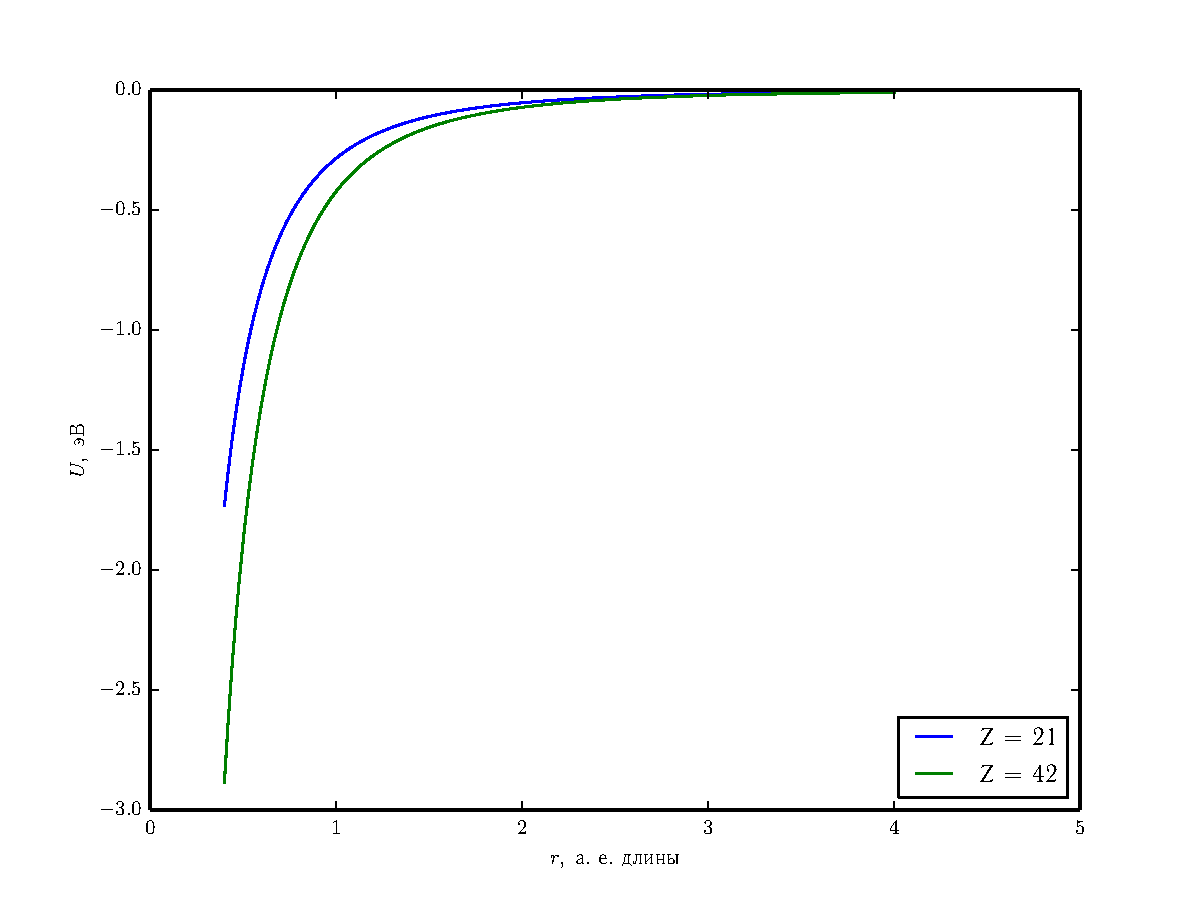
\includegraphics[width=.55\textwidth]{Z_21_42} \\
%  \parbox{.49\textwidth}{\caption{Решение уравнения Томаса--Ферми
%  \eqref{eq:7}} \label{fig:1}}
%  \parbox{.49\textwidth}{\caption{Зависимость потенциальной энергии
%  электрона \( U \) от координаты \( r \)} \label{fig:2}} 
%  \end{figure}
%  \newpage
%  \section{Листинги программ}
%  \lstinputlisting[language=c++,
%    caption=Расчёт решения уравнения Томаса-Ферми]{code/tf.cpp}
%  
%  \vspace{1.5em}
%  \lstinputlisting[language=python,caption=Построение графиков]{code/plots.py}
  
\end{document}
